\documentclass[a4paper]{article}

% Includes packages relevant to Senior Lab

% character set specifications
\usepackage[english]{babel}
\usepackage[utf8]{inputenc}

% increased vertical spacing for tables
\newcommand\topVspace{\rule{0pt}{2.6ex}}      
\newcommand\bottomVspace{\rule[-1.2ex]{0pt}{0pt}} 

% extra unicode characters
\DeclareUnicodeCharacter{3BC}{\(\mu\)}
\DeclareUnicodeCharacter{3C1}{\(\rho\)}
\DeclareUnicodeCharacter{2080}{\(_0\)}
\DeclareUnicodeCharacter{2081}{\(_1\)}
\DeclareUnicodeCharacter{2082}{\(_2\)}
\DeclareUnicodeCharacter{3B5}{\(\epsilon\)}
\DeclareUnicodeCharacter{3B1}{\(\alpha\)}

% SI Units
\usepackage{siunitx}

% extra SI units
\DeclareSIUnit\gauss{G}

% enable scientific notation
\sisetup{scientific-notation = engineering, exponent-to-prefix}

% draw pretty lines
\usepackage{tikz}
\usetikzlibrary{datavisualization}
\usepackage{circuitikz}

% manual tabbing
\setlength{\parindent}{0pt}
\def\qq{\qquad}

% include graphics
\usepackage{graphicx}

% increased control over figure placement
\usepackage{float}

% box answers
\usepackage{tcolorbox}

% enable multiple section levels
\usepackage{titlesec}

% define `\subsubsubsection` command
\titleclass{\subsubsubsection}{straight}[\subsection]
\newcounter{subsubsubsection}[subsubsection]
\renewcommand\thesubsubsubsection{\thesubsubsection.\arabic{subsubsubsection}}
\titleformat{\subsubsubsection}
        {\normalfont\normalsize\bfseries}{\thesubsubsubsection}{1em}{}
\titlespacing*{\subsubsubsection}
{0pt}{3.25ex plus 1ex minus .2ex}{1.5ex plus .2ex}
\setcounter{secnumdepth}{4}

% get align environment (among other things)
\usepackage{amsmath}

% bold in math mode
\usepackage{bm}

% get \mathbb (among other things)
\usepackage{amssymb}

\usepackage{array}

% plotting
\usepackage{pgfplots}

% enable external references
\usepackage{hyperref}

% include code
\usepackage[cache=false]{minted}
\setminted{linenos, frame=lines, texcomments}

% adjust margins of individual pages (for shoving figures into place)
\usepackage{changepage}

% rotate figures
\usepackage{rotating}


\usepackage{caption}
\renewcommand{\thetable}{\arabic{section}.\arabic{table}}
\newcommand\T{\rule{0pt}{2.6ex}}       % Top strut
\newcommand\B{\rule[-1.2ex]{0pt}{0pt}} % Bottom strut

\title{PHY 4210-01 Senior Lab \\Lab P2: Electron Spin Resonance}

\author{Sarah Arends \\ 
        Jacquelyne Miksanek \\
        Ryan Wojtyla \\ \\
        Instructor: Jerry Collins}

\date{March 28, 2019}

\begin{document}
\maketitle 

\begin{abstract}
%physics of experiment
%apparatus used
%what was measured
%Results

\qq The Lande factor, $g_s$, (or the gyromagnetic ratio of spin) for the
electron was determined through the use of electron spin resonance and
Helmholtz coils. The g-factor of a diphenyl-picryl-hydrazyl (DPPH) sample was
obtained following the measurement of the frequency dependence of the
resonance field. The line width of the resonance signal was then calculated.

\end{abstract}

\newpage

\tableofcontents

\newpage

\section{Data Analysis}
%Graphs, figures, and tables with captions
%Results with error analysis
%Calculate discrepancies from theory
\subsection{Frequency Dependence of Resonance Field}

\qq Voltage was compared to frequency to obtain a graphical
relationship of the frequency dependence of the resonance field. The
amplitude voltage was obtained by measuring the peak-to-peak voltage
from the oscilloscope and dividing it in half. The peak of
\ref{FrequencyDependence} is the specific resonance frequency for the field.
\begin{figure}[H]
\centering
% uncomment the line below to add image
%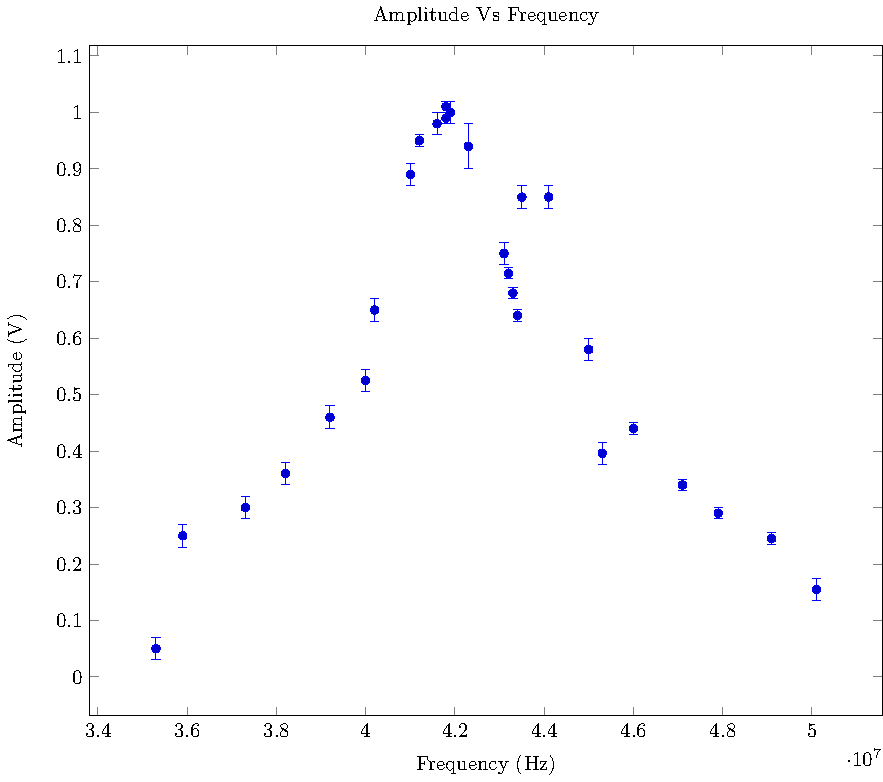
\includegraphics[scale=2.0]{freq_depen.png}
\captionof{figure}{Graphic representation of the frequency dependence
  of the resonance field.}
\label{FrequencyDependence}
\end{figure}

\subsection{Propagation of Uncertainty in the Frequency Dependence of the Resonance Field}

\subsection{Experimental Value of Gyromagnetic Ratio}
\qq The gyromagnetic ratio is calculated using the following equation, where $\nu$ is the frequency, $h$ is Planck's constant, $\mu_B$ is the Bohr magneton, and $B_0$ is the magnetic field strength.
\begin{equation}
\label{eq:exp_gs}
g_s = \frac{h \times \nu}{\mu_B \times B_0}
\end{equation} 

\qq The magnetic field used in calculating equation \ref{eq:exp_gs} must be calculated as well. It is determined from the measured current using equation \ref{eq:exp_B}, where $\mu_0 = 4 \pi \times 10^{-7} \frac{Vs}{Am}$, the number of turns is $n=320$, and the radius of the coils is $r=6.8cm$.
\begin{equation}
\label{eq:exp_B}
B_0 = \mu_0 \left( \frac{4}{5} \right) ^{3/2} \times \frac{n}{r} \times I
\end{equation}

\qq Rather than measuring the current directly, the current is calculated by measuring the voltage drop across a resistor, of which the resistance is also measured. This calculation is shown below in equation.
\begin{equation}
\label{eq:exp_I}
I = \frac{V}{R}
\end{equation}

\qq By substituting equation \ref{eq:exp_I} into \ref{eq:exp_B}, and then substituting equation \ref{eq:exp_B} into equation \ref{eq:exp_gs}, we arrive at an expression for the gyromagnetic ratio in terms of known constants and measured quantities. This final expression is shown in equation \ref{eq:exp_gs_combined}.
\begin{equation}
\label{eq:exp_gs_combined}
g_s = \frac{h \times \nu}{\mu_B \times \left( \mu_0 \left( \frac{4}{5} \right) ^{3/2} \times \frac{n}{r} \times \frac{V}{R} \right) }
\end{equation}

\subsection{Propagating Uncertainty in Gyromagnetic Ratio}
\qq The error in the experimental value of the gyromagnetic ratio is determined by propagating uncertainty in equation \ref{eq:exp_gs_combined}. There are no uncertainties associated with fundamental constants such as $h$, $\mu_B$, and $\mu_0$. It is assumed that the number of coil turns, $n$, also has no associated uncertainty because it was reported in the manual as such. The uncertainty in the radius is constant for all measurements, ,but the frequency, voltage, and resistance will differ for each measurement. Equation \ref{eq:delta_gs} shows this error propagation.

\begin{equation}
\label{eq:delta_gs}
\delta g_s = g_s \times 
              \sqrt {
              		  \left( \frac{\delta \nu}{\nu} \right) ^2
              		+ \left( \frac{\delta r}{r} \right) ^2
              		+ \left( \frac{\delta V}{V} \right) ^2
              		+ \left( \frac{\delta R}{R} \right) ^2
					} \\
\end{equation}

An example calculation for the value of $g_s$ and its propagated uncertainty is shown below for a measurement taken with the large coil:

\begin{align*}
g_s &= \\
    &= 1.93 \\
\end{align*}

\begin{align*}
\delta g_s &=
		   g_s \times 
              \sqrt {
              		  \left( \frac{1.00 \times 10^4 \text{Hz}}{3.00 \times 10^47 \text{Hz}} \right) ^2
              		+ \left( \frac{0.5 \text{cm}}{6.7 \text{cm}} \right) ^2
              		+ \left( \frac{0.1 \text{V}}{2 \text{V}} \right) ^2
              		+ \left( \frac{0.1 \Omega}{1.7 \Omega} \right) ^2
					} \\
		  &= g_s \times 
              \sqrt {
              		  \left( num \right) ^2
              		+ \left( 0.006 \right) ^2
              		+ \left( num \right) ^2
              		+ \left( num \right) ^2
					}
\end{align*}

\subsection{Determining Line Width of Resonance Signal}
\qq 

\section{Results}
%Discuss results and uncertainties
%Compare results with theory
%Approximations to theory
\qq

\subsection{Discrepancy in Gyromagnetic Ratio}
\qq 

\subsection{Discrepancy in Line Width}
\qq 

\section{Conclusion}
%Brief summary, discussion of results and theory
\qq 

\section{Appendices}

\subsection{Appendix A: Data}

\subsection{Appendix B: Source Code}

\end{document}
